\chapter{Кинематика твердого тела. Плоское движение. Определение кинематических
характеристик движения: траектории движения скорости и ускорения
произвольной точки тела. Понятие о мгновенном центре скоростей.}

Движение твердого тела называется плоским, если все точки тела перемещаются в
плоскостях, параллельных некоторой неподвижной плоскости. Примером плоского
движения тела может служить качение цилиндра по горизонтальной плоскости.

\begin{minipage}{.4\textwidth}
    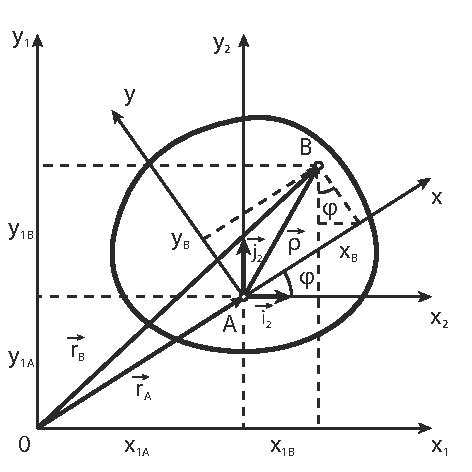
\includegraphics[width=\textwidth]{26_01}
\end{minipage}
\begin{minipage}{.55\textwidth}
Пусть система координат \( Ox_1y_1 \) является неподвижной системой, а система
координат \( Ax_2y_2 \), имеющая начало в произвольной точке \( A \) плоской
фигуры, движется поступательно. Систему координат \( Axy \) жестко свяжем с
плоской фигурой.

Радиус-вектор \( \vec{r}_B \), определяющий положение точки \( B \) относительно
\( Ox_1y_1 \), можно задать при помощи векторов \( \vec{r}_A \), определяющего
положение точки \( A \) в \( Ox_1y_1 \), и \( \vec{\rho} \), определяющего
положение точки \( B \) в \( Ax_2y_2 \): \(\vec{r}_B = \vec{r}_A + \vec{\rho}\).

Зная координаты \( x_{1A} \) и \( y_{1A} \) точки \( A \) и координаты \( x_B \)
и \( y_B \) точки \( B \) в \( Axy \), а также угол \( \phi \) между осями
\( Ax_2 \) и \( Ax \), можно определить координаты \( x_{1B} \) и \( y_{1B} \)
точки \( B \):
\end{minipage}
\[
    \left\{ \begin{array}{l}
        x_{1B} = x_{1A}(t) + x_B\cos\phi(t) - y_B\sin\phi(t), \\
        y_{1B} = y_{1A}(t) + x_B\sin\phi(t) + y_B\cos\phi(t).
    \end{array} \right.
\]
Продифференцировав по времени, получим проекции скорости точки \( B \):
\[
    \left\{ \begin{array}{l}
        \dot{x}_{1B} = \dot{x}_{1A} - x_B\dot{\phi}\sin\phi -
        y_B\dot{\phi}\cos\phi, \\
        \dot{y}_{1B} = \dot{y}_{1A} + x_B\dot{\phi}\cos\phi +
        y_B\dot{\phi}\sin\phi.
    \end{array} \right.
\]
К этому результату можно прийти, продифференцировав выражение для
\( \vec{r}_B \) по времени: \( \ds \der{\vec{r}_B}{t} = \der{\vec{r}_A}{t} +
\der{\vec{\rho}}{t} \). Заметим, что \( \ds \vec{v}_B = \der{\vec{r}_B}{t} \),
\( \ds \vec{v}_A = \der{\vec{r}_A}{t} \), а \( \ds \vec{v}_{BA} =
\der{\vec{\rho}}{t} \) -- это скорость точки \( B \) относительно \( Ax_2y_2 \),
то есть относительная скорость, которую можно представить в виде:
\( \vec{v}_{BA} = \vec{\omega}\times\vec{\rho} \).

Тогда скорость точки \( B \) имеет вид: \( \vec{v}_B = \vec{v}_A +
\vec{\omega}\times\vec{\rho} \).

Найдем ускорения точки плоской фигуры продифференцировав по времени последнее
выражение:
\[
    \der{\vec{v}_B}{t} = \der{\vec{v}_A}{t} + \der{\vec{\omega}}{t}\times
    \vec{\rho} + \vec{\omega}\times\der{\vec{\rho}}{t}.
\]
 
В этом соотношении \( \ds \der{\vec{v}_B}{t} = \vec{a}_B \) и
\( \ds \der{\vec{v}_A}{t} = \vec{a}_A \) -- ускорения точек \( A \) и \( B \),
\( \ds \der{\vec{\omega}}{t} = \vec{\eps} \) -- угловое ускорение, а
\( \ds \der{\vec{\rho}}{t} = \vec{v}_{BA} \) -- относительная скорость. Таким
образом, ускорения точек \( A \) и \( B \) связаны формулой:
\[
    \vec{a}_B = \vec{a}_A + \vec{\eps}\times\vec{\rho} +
    \vec{\omega}\times\vec{v}_{BA}.
\]

\section{Мгновенный центр скоростей}

\begin{minipage}{.4\textwidth}
    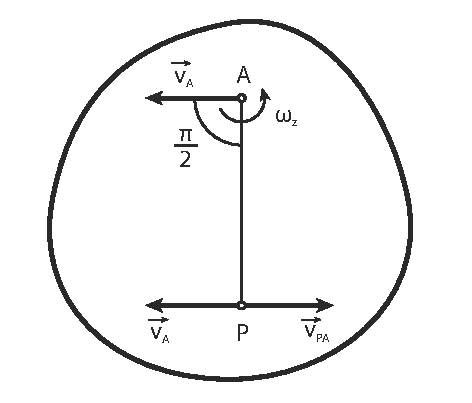
\includegraphics[width=\textwidth]{26_02}
\end{minipage}
\begin{minipage}{.55\textwidth}
Мгновенным центром скоростей называется точка плоской фигуры, скорость которой в
данный момент времени равна нулю. Докажем теорему о существовании мгновенного
центра скоростей: если угловая скорость плоской фигуры отлична от нуля, то
мгновенный центр скоростей существует. Пусть скорость \( \vec{v}_A \)
произвольной точки плоской фигуры отлична от нуля. По знаку угловой скорости
\( \omega = \dot{\phi} \) определяем направление вращения плоской фигуры вокруг
точки \( A \) и в этом направлении откладываем от точки \( A \) отрезок
\( AP = v_a/\omega \) перпендикулярно скорости \( \vec{v}_A \).
Докажем, что скорость полученной точки \( P \) равна нулю, то есть эта точка и
есть мгновенный центр скоростей. Имеем: \( \vec{v}_P = \vec{v}_A +
\vec{v}_{PA} \).
\end{minipage}
 
Так как скорость \( \vec{v}_{PA} \) перпендикулярна \( AP \), то вектор
\( \vec{v}_{PA} \) параллелен \( \vec{v}_A \). Кроме того, в соответствии с
правилом построения отрезка \( AP \) векторы \( \vec{v}_A \) и
\( \vec{v}_{PA} \) имеют противоположные направления. Модуль \( \vec{v}_{PA} \)
равен: \( v_{PA} = \omega\cdot AP = v_A/\omega\cdot\omega = v_A \).

Два вектора, равных по величине и противоположно направленных, в сумме дают нуль.
Следовательно, скорость точки Р равна нулю, и эта точка и есть мгновенный центр
скоростей.

\newpage % ---------------------------------------------------------------------
